%!TEX root = ./main.tex


The final step requires to add a final cost term to the OCP in \eqref{eq:ocp}, enabling the computation using the trained neural network. Thus the new OCP becomes:

\begin{equation}
\label{eq:ocp_final}
\begin{aligned}
    \min_{\mathbf{X}, \mathbf{U}} \quad & \sum_{k=0}^{M-1} \left( (\mathbf{x}_k - \mathbf{x}_{targ})^\top \mathbf{W}_x (\mathbf{x}_k - \mathbf{x}_{targ}) + (u_k - u_{targ})^\top \mathbf{W}_u (u_k - u_{targ}) \right) + J(\mathbf{x}_M) \\
    \text{subject to} \quad & \mathbf{x}_0 = \mathbf{x}_{init} \\
    & \mathbf{x}_{k+1} = \mathbf{f}(\mathbf{x}_k, u_k), \quad k = 0, \dots, M-1
\end{aligned}
\end{equation}
\vspace{\baselineskip}

\noindent Where \(J(\mathbf{x}_M)\) is the final cost computed using the trained neural network, given the final state \(\mathbf{x}_M\) at the end of the horizon. \\

\noindent The objective of this part is to compare three different MPC controllers:
\begin{itemize}[noitemsep]
    \item Without final cost and horizon M < N
    \item With final cost computed using the network cost function and horizon M < N
    \item Without final cost and horizon M + N
\end{itemize} 

\noindent Where N is the full horizon length used during the dataset generation.

\noindent
It is to be expected to see the last two controllers perform similarly, while the first one would be less effective, since it does not account for the final cost and has a shorter horizon.\\

\noindent The first operation is to create a CasADi function that implements the neural network trained in the previous section. This function takes into account the normalization steps used during training. So it takes as input the state \(\mathbf{x}\), normalizes it  \(\mathbf{x}_{norm}\) and outputs the estimated cost \(J(\mathbf{x}_{norm})\) by re-converting it back from logarithmic scale.

\noindent To speed up the MPC computation and obtain better results, a warm-starting strategy has been implemented. At each MPC iteration, the previous solution is used as an initial guess for the next optimization problem. Specifically, the state and control trajectories from the previous solution are shifted forward by one time step, and the last state is repeated to fill in the gap created due to the shift. This approach helped providing a good initial guess for the solver and showed better convergence speed and solution quality. 
\\
The values chosen for the MPC controllers are:
\begin{itemize}[noitemsep]
    \item Short-Horizon length: \(M = 14\) 
    \item Long-Horizon length: \(M + N = 114\)
\end{itemize}

\noindent Obviously, all the hyperparameters used in the OCP definition are the same as in \eqref{eq:ocp}.\\

\noindent With all of this set up, the three MPC controllers are tested on 30 randomly sampled initial conditions:

\begin{itemize}[noitemsep]
    \item Joint 1 position ($q_1$): uniformly sampled in $[-\pi, \pi]$
    \item Joint 2 position ($q_2$): uniformly sampled in $[-0.8\pi, 0.8\pi]$
    \item Angular velocities ($\dot{q}_1, \dot{q}_2$): uniformly sampled in $[-1.0, 1.0]$ rad/s 
\end{itemize}

\newpage

\noindent Two examples of the trajectories obtained with the three different MPC controllers are shown in Figure \ref{fig:fase3_traj} and Figure \ref{fig:run_bella}, by using the same initial condition: 

\begin{itemize}
    \item Initial Conditions 1: \(\mathbf{x}_{init} = [-0.820,\  -0.60,\    0.990,\  -0.830]^\top\)
    \item Initial Condition 2: \(\mathbf{x}_{init} = [-0.237,\ 0.612,\ 0.732,\ 0.596 ]^\top\)
\end{itemize}

\begin{figure}[H]
    \centering
    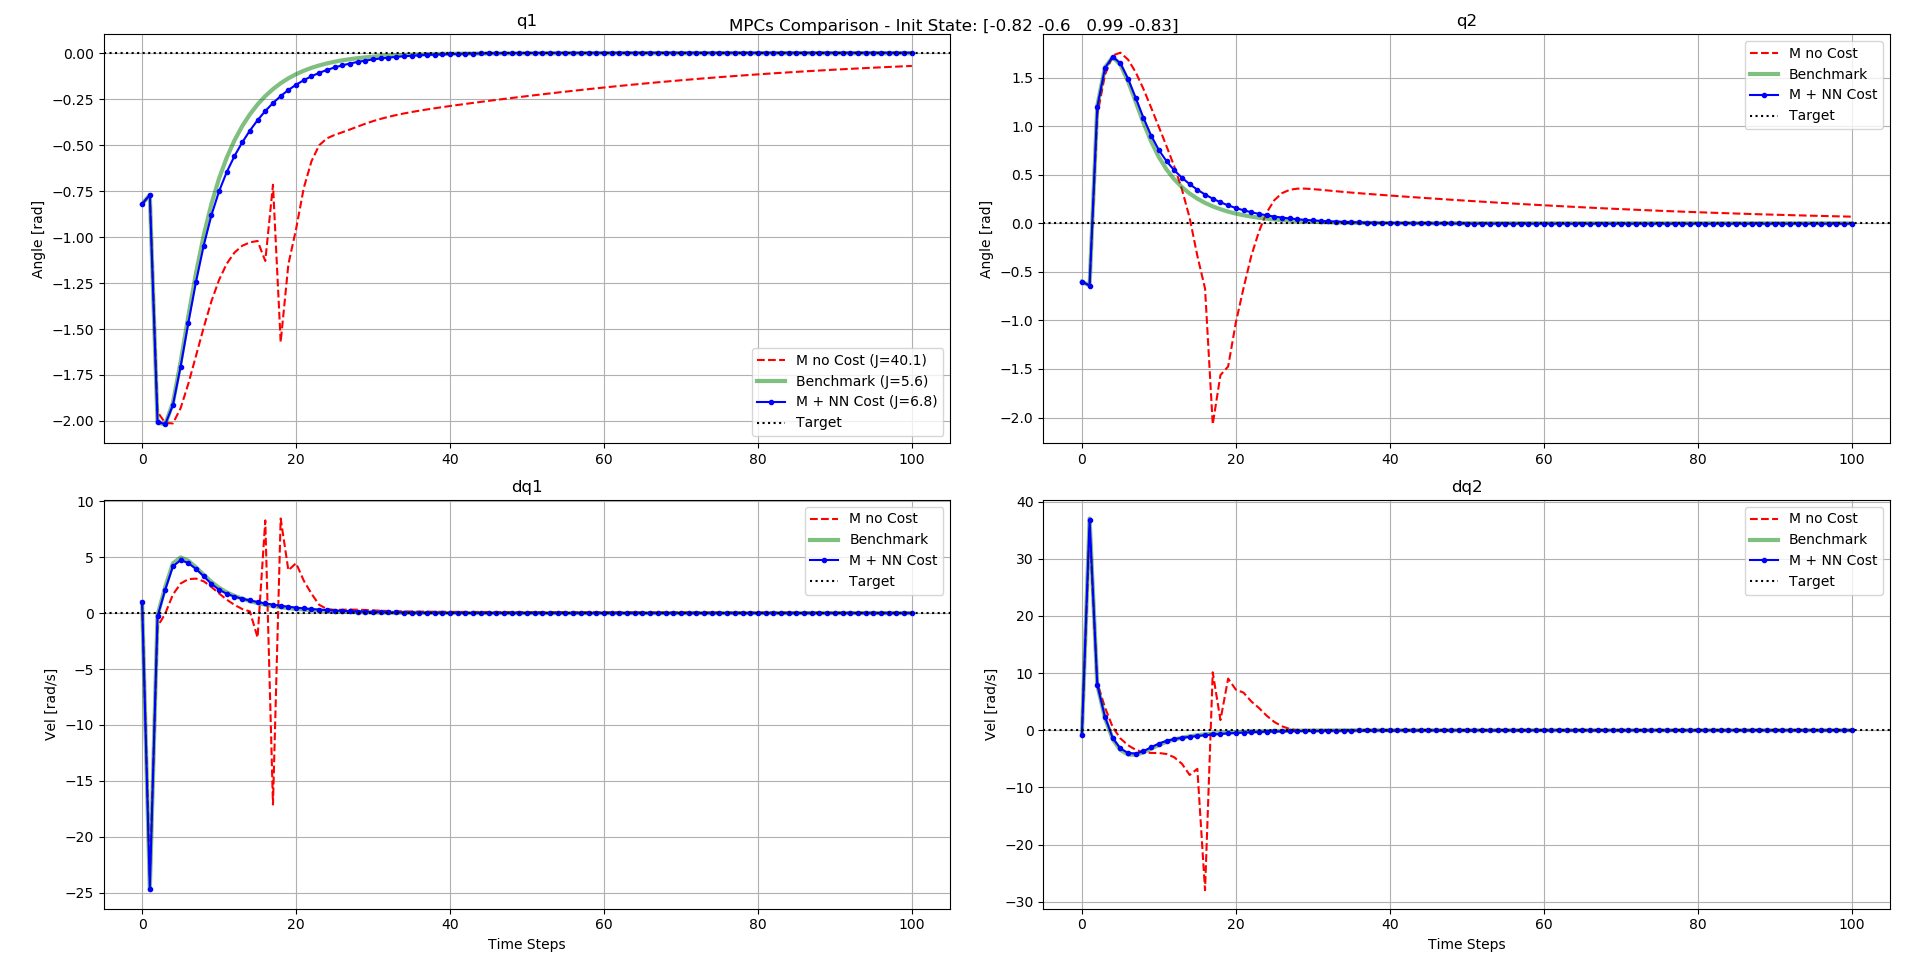
\includegraphics[width=1\textwidth]{pics/mpcs.png} 
    \caption{Trajectories obtained with the three different MPC controllers using initial conditions 1.}
    \label{fig:fase3_traj}
\end{figure}

\begin{figure}[H]
    \centering
    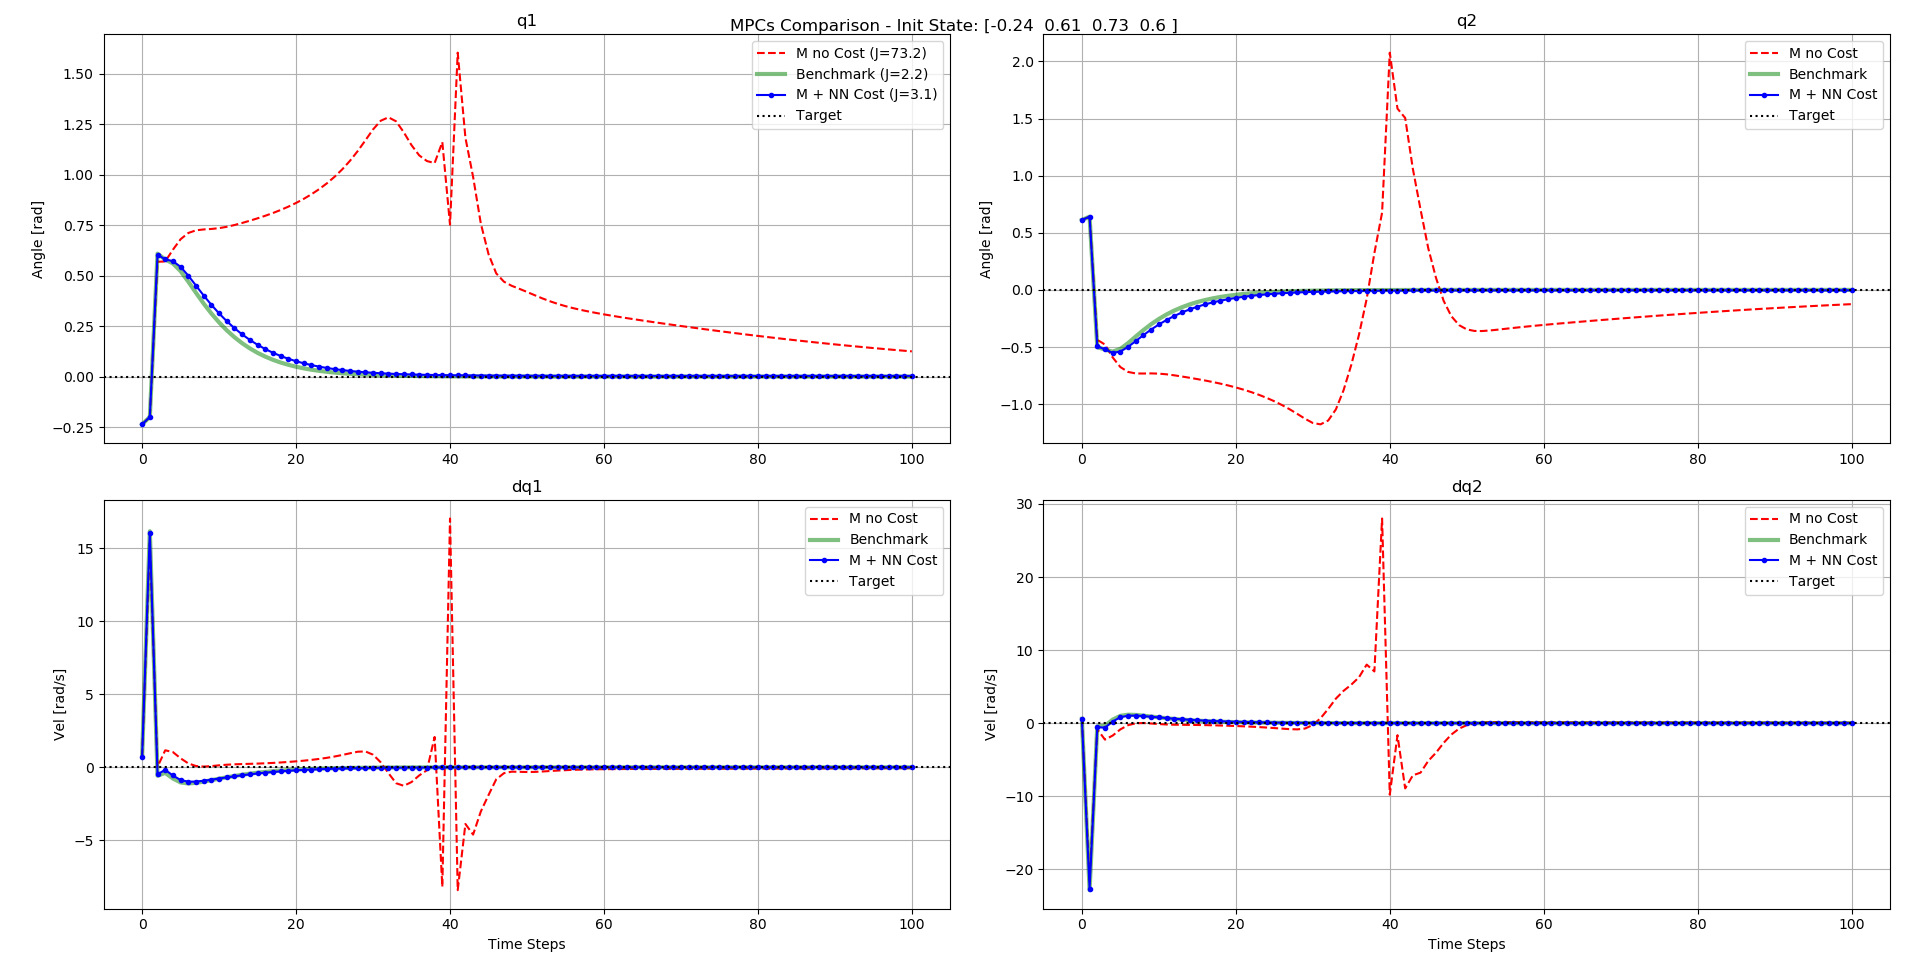
\includegraphics[width=1\textwidth]{pics/run_bella.png} 
    \caption{Trajectories obtained with the three different MPC controllers using initial condition 2.}
    \label{fig:run_bella}
\end{figure}
\newpage

\noindent As can be seen, in both cases the controller with final cost (blue) and the one with the long horizon (green) perform similarly, while the one without final cost and the long horizon (red) performs worse, as expected.\\

\noindent By following the links, the videos of the trajectories above can be seen: 
\begin{itemize}[noitemsep]
    \item Initial Conditions 1: \url{https://youtu.be/dTzMtQ39pxc}

        \item Initial Conditions 2: \url{https://youtu.be/vgQT7q9oPIk}
\end{itemize}


\noindent Some multiple run trajectories are reported in: \url{https://youtu.be/99hOP7C9648}. The initial states of these examples are: 
\begin{itemize}[noitemsep]
    \item \(\mathbf{x}_{init} = [ \pi, 0.0,  0.0   ,  0.0   ]^\top\)
    \item \(\mathbf{x}_{init} = [1.1415, 2.827, 0.5, -0.9999 ]^\top\)
    \item \(\mathbf{x}_{init} = [-2, -0.60, 0.3, -0.83 ]^\top\)
    \item \(\mathbf{x}_{init} = [0.1, -2.60, 0.6, -0.23 ]^\top\)
\end{itemize}

\noindent To compare the three controllers quantitatively, the total cost is computed over the 30 runs. However, the cost defined in \eqref{eq:ocp_final} turned out to be not very informative, since some times the trajectories obtained were clearly better in the case of the MPC with final cost or long horizon, but their total cost was higher with respect to the short horizon case. This is due to the fact that the cases with final cost or long horizon tend to reach the target state more aggressively. This implies high values of the state and control errors during the initial part of the trajectory. This difference value is then squared, making the total cost higher. On the other hand the case with short horizon tends to reach the target in more time, resulting in lower errors  peaks and thus a lower total cost.

For this reason, the comparison has been held on a different cost, based on  metrics. This is not an optimal solution, the OCP cost should have been redefined, but given the time constraints, it has been set to proceed this way. The results obtained in this manner are still meaningful and of interest.\\

\noindent The new cost has been computed from the one in \eqref{eq:ocp_final} by applying the square root to the state and control error terms, thus obtaining a cost that penalizes linearly the errors instead of quadratically. A weight $w_t$ which is increased linearly with time has also been implemented, to further penalize the errors at the end of the trajectory. Thus the new cost becomes:

\begin{gather}
\label{eq:realized_cost_metrics}
    L(\mathbf{x}_k, \mathbf{u}_k) = \sqrt{(\mathbf{x}_k - \mathbf{x}_{ref})^T W_x (\mathbf{x}_k - \mathbf{x}_{ref})} + \sqrt{(\mathbf{u}_k - \mathbf{u}_{ref})^T W_u (\mathbf{u}_k - \mathbf{u}_{ref})} \\[10pt]
    w_t = \left( \frac{k+1}{N} \right) \\[10pt]
    J_{comparison} = \sum_{k=0}^{N-1}  w_t\cdot L(\mathbf{x}_k, \mathbf{u}_k)
\end{gather}

\noindent Where:
\begin{itemize}[noitemsep]
    \item \(L(\mathbf{x}_k, \mathbf{u}_k)\) is the instantaneous cost at time step \(k\)
    \item \(J_{comparison}\) is the total cost used for comparison
    \item \(N\) is the total number of time steps in the trajectory
\end{itemize}

\noindent A second metric used for the comparison, is the time taken by each pendulum to reach the target state within a certain state threshold. This was done by monitoring if the Euclidean distance between the current state $\mathbf{x}_k$ and the target equilibrium $\mathbf{x}_{ref}$ was below an arbitrary threshold of $0.08$.\\

\noindent The results obtained over the 30 simulations are reported in Table \ref{tab:mpc_results}.


\noindent As can be seen 25 times out of 30, the MPC with final cost performed better than the short horizon one without final cost. This means that $83\%$ of the times the use of the learned final cost improved the performance. In the other 5 cases, the MPC with the final cost performed significantly worse, this is probably due to some limitations in the neural network that can be probably be solved by better training.\\

\noindent By analyzing the time taken to reach the target state, the MPC with short horizon and without final cost was essentially unable to reach the target within the treshold in most of the cases, while the MPC with final cost reached the target in 27 cases out of 30 (90\% of success rate). This shows that the use of the learned final cost significantly improves the controller's ability to reach the desired state within a reasonable time frame.\\

\noindent NOTE: when the time is -1 it means that the controller was unable to reach the target within the distance threshold.

\begin{table}[h!]
\centering
\caption{Comparative performance analysis of MPC strategies across 30 random initial states. Case 1: Short horizon ($M=14$) without terminal cost. Case 2: Short horizon ($M=14$) with Learned NN Terminal Cost. Case 3: Long horizon benchmark ($N+M=114$). Negative time values ($-1.00$) indicate a failure to converge within the distance threshold.}
\label{tab:mpc_results}
\resizebox{\textwidth}{!}{%
\begin{tabular}{c|>{\centering\arraybackslash}p{4.5cm}|cc|cc|cc}
\hline
\textbf{Run} & \textbf{Initial State $[q_1, q_2, \dot{q}_1, \dot{q}_2]$} & \multicolumn{2}{c|}{\textbf{Case 1 (M=14)}} & \multicolumn{2}{c|}{\textbf{Case 2 (M+NN)}} & \multicolumn{2}{c}{\textbf{Case 3 (N+M=114)}} \\
\# & [rad, rad, rad/s, rad/s] & Cost & Time [s] & Cost & Time [s] & Cost & Time [s] \\ \hline
1  & [1.53, 1.32, 0.28, 0.58]   & 23.846 & 4.95  & 16.00  & 2.10  & 12.607 & 1.75  \\
2  & [0.12, 0.95, 0.18, 0.40]   & 57.763 & -1.00 & 4.24   & 1.55  & 3.191  & 1.40  \\
3  & [-2.68, 0.69, 0.99, -0.00] & 36.308 & -1.00 & 11.75  & 1.85  & 10.661 & 1.65  \\
4  & [-0.56, -0.75, -0.31, -0.50]& 39.765 & -1.00 & 6.13   & 1.70  & 5.086  & 1.50  \\
5  & [-1.27, -1.59, -0.82, 0.90] & 20.865 & 4.65  & 3.84   & 1.45  & 3.264  & 1.35  \\
6  & [-2.82, 2.32, -0.28, 0.07]  & 33.267 & -1.00 & 13.25  & 1.95  & 8.315  & 1.65  \\
7  & [1.36, 0.62, 0.19, -0.08]   & 24.683 & -1.00 & 9.52   & 1.90  & 7.565  & 1.60  \\
8  & [0.81, 0.56, -0.80, 0.41]   & 37.060 & -1.00 & 7.23   & 1.75  & 5.725  & 1.55  \\
9  & [0.41, 1.61, -0.72, -0.05]  & 15.513 & 4.05  & 2.93   & 1.25  & 2.238  & 1.15  \\
10 & [-0.76, -1.87, 0.71, -0.94] & 34.390 & -1.00 & 83.85  & 4.05  & 2.533  & 1.25  \\
11 & [2.03, -0.72, -0.69, -0.98] & 28.864 & -1.00 & 10.52  & 1.85  & 9.161  & 1.60  \\
12 & [1.35, -0.84, 0.54, -0.85]  & 28.764 & -1.00 & 157.57 & -1.00 & 7.811  & 1.60  \\
13 & [2.75, -0.41, 0.64, 0.24]   & 34.007 & -1.00 & 65.18  & -1.00 & 11.137 & 1.70  \\
14 & [1.83, -1.24, 0.05, 0.75]   & 31.062 & -1.00 & 8.96   & 2.00  & 6.909  & 1.60  \\
15 & [1.74, 1.24, 0.65, -0.38]   & 25.747 & -1.00 & 4.02   & 1.45  & 3.936  & 1.40  \\
16 & [-2.08, -0.01, -0.25, 0.41] & 29.259 & -1.00 & 10.25  & 1.80  & 9.219  & 1.65  \\
17 & [-2.21, -1.59, 0.40, -0.45] & 26.836 & -1.00 & 5.84   & 1.60  & 5.615  & 1.50  \\
18 & [-1.44, -1.17, 0.60, 0.61]  & 34.476 & -1.00 & 7.17   & 1.75  & 6.043  & 1.60  \\
19 & [-2.89, 1.94, -0.09, -0.69] & 36.587 & -1.00 & 15.19  & 2.35  & 32.760 & 2.05  \\
20 & [2.43, -0.54, 0.04, -0.34]  & 36.559 & -1.00 & 15.52  & 1.95  & 10.134 & 1.65  \\
21 & [2.07, -1.98, 0.66, -0.82]  & 34.207 & -1.00 & 216.30 & -1.00 & 6.180  & 1.55  \\
22 & [-1.41, -0.37, -0.60, -0.10]& 25.576 & -1.00 & 9.33   & 1.85  & 7.981  & 1.60  \\
23 & [-0.71, 1.55, -0.98, 0.62]  & 5.506  & 1.90  & 1.41   & 0.60  & 0.859  & 0.60  \\
24 & [2.90, 2.04, 0.18, 0.92]    & 30.096 & -1.00 & 7.16   & 1.65  & 6.141  & 1.55  \\
25 & [1.67, 1.84, -0.95, 0.89]   & 19.431 & 4.50  & 4.09   & 1.45  & 3.271  & 1.35  \\
26 & [-0.06, 1.59, 0.09, -0.28]  & 12.398 & 3.60  & 2.44   & 1.15  & 1.784  & 1.05  \\
27 & [2.48, 0.74, -0.15, 0.26]   & 37.187 & -1.00 & 53.89  & 3.15  & 9.047  & 1.65  \\
28 & [-2.71, 0.05, 0.01, 0.74]   & 31.776 & -1.00 & 11.33  & 1.85  & 10.126 & 1.65  \\
29 & [-0.51, -0.83, -0.41, -0.65]& 44.524 & -1.00 & 5.79   & 1.65  & 4.802  & 1.50  \\
30 & [2.55, 0.69, 0.14, -0.14]   & 33.484 & -1.00 & 14.49  & 1.95  & 9.994  & 1.70  \\ \hline
\end{tabular}%
}
\end{table}